\documentclass[longbibliography,nofootinbib,twocolumn]{revtex4-1}

\newcommand{\kms}{NuCypher KMS}

\usepackage{listings}
\usepackage{graphicx}
\usepackage{amsmath}
\usepackage[margin=5pt]{subfig}
\usepackage[usenames]{color}

\renewcommand{\baselinestretch}{1.4}
\setlength{\parskip}{1em}
\definecolor{darkgreen}{rgb}{0.00,0.50,0.25}
\definecolor{darkblue}{rgb}{0.00,0.00,0.67}
\newcommand{\figref}[1]{Fig.~\ref{#1}}
\usepackage[breaklinks,pdftitle={NuCypher KMS: Mining}, pdfauthor={Michael Egorov},colorlinks,urlcolor=blue,citecolor=darkgreen,linkcolor=darkblue]{hyperref}
\graphicspath{{pdf/}}

\usepackage[T1]{fontenc}
\usepackage{lmodern}
\lstset{
    basicstyle=\ttfamily,
    basewidth={0.5em, 0.5em},
    columns=fullflexible,
}

\begin{document}

\title{\kms: Mining}

\author{Michael Egorov}
\email{michael@nucypher.com}
\affiliation{NuCypher}

\begin{abstract}
    This paper describes mining mechanisms and economics in \kms.
    It includes inflation rates, mechanisms to incentivise long-term stakers
    and estimates of number of coins generated by nodes running in typical modes.
    Also, optimal strategies for stakers who may be affected by market volatility are proposed.
\end{abstract}

\date{\today}
\maketitle

\section{Motivation}

In future, \kms~will probably be fully paid by network fees.
But initially, when the adoption isn't yet high, miners who run the nodes necessary for network operation and keep re-encryption keys,
will need to be subsidised.
This will be done through inflation schedule, where all the inflation is given back to miners.

Distribution of rewards should have the following properties:
\begin{itemize}
    \item All the inflation is distributed to stakers who run the nodes, proportionally to the stake;
    \item Amount of work (and, hence, the fees) is proportional to stake also;
    \item Stakers are incentivized (by a higher reward rate) to run long-term nodes;
    \item High inflation doesn't depreciate the price in order to keep liquidity good for new stakers;
    \item Stakers are incentivized to stay online all the time.
\end{itemize}

In the paper we address all these points, calculate expected earnings of miners who run nodes and devise optimal mining strategies.

\section{Historical examples of inflation}

Let's review inlation schedules of different cryptocurrency projects:
DASH~\cite{dash:whitepaper} and ZCash~\cite{zcash}.

Dash has a hybrid of Proof-of-Work (POW) and Proof-of-Stake (POS).
It has $45\%$ of inflation going to POW miners, $45\%$ to staking master nodes and $10\%$ is reserved for budget proposals~\cite{dash:emission}.
After the first year, its emission was $18.42\%$ APR, decreasing by $1/14$ every $383$ days.
With this setting, $60\%$ of DASH coins are locked in masternodes for staking, according to the node statistics.
It's unclear how inflation rate affects the price (and if it does here), but the useful data point is that there are $60\%$ of coins locked for staking.
Perhaps, that is something to expect in a network where staking is an option.

% TODO: replot in a more reasonable shape
\begin{figure}
    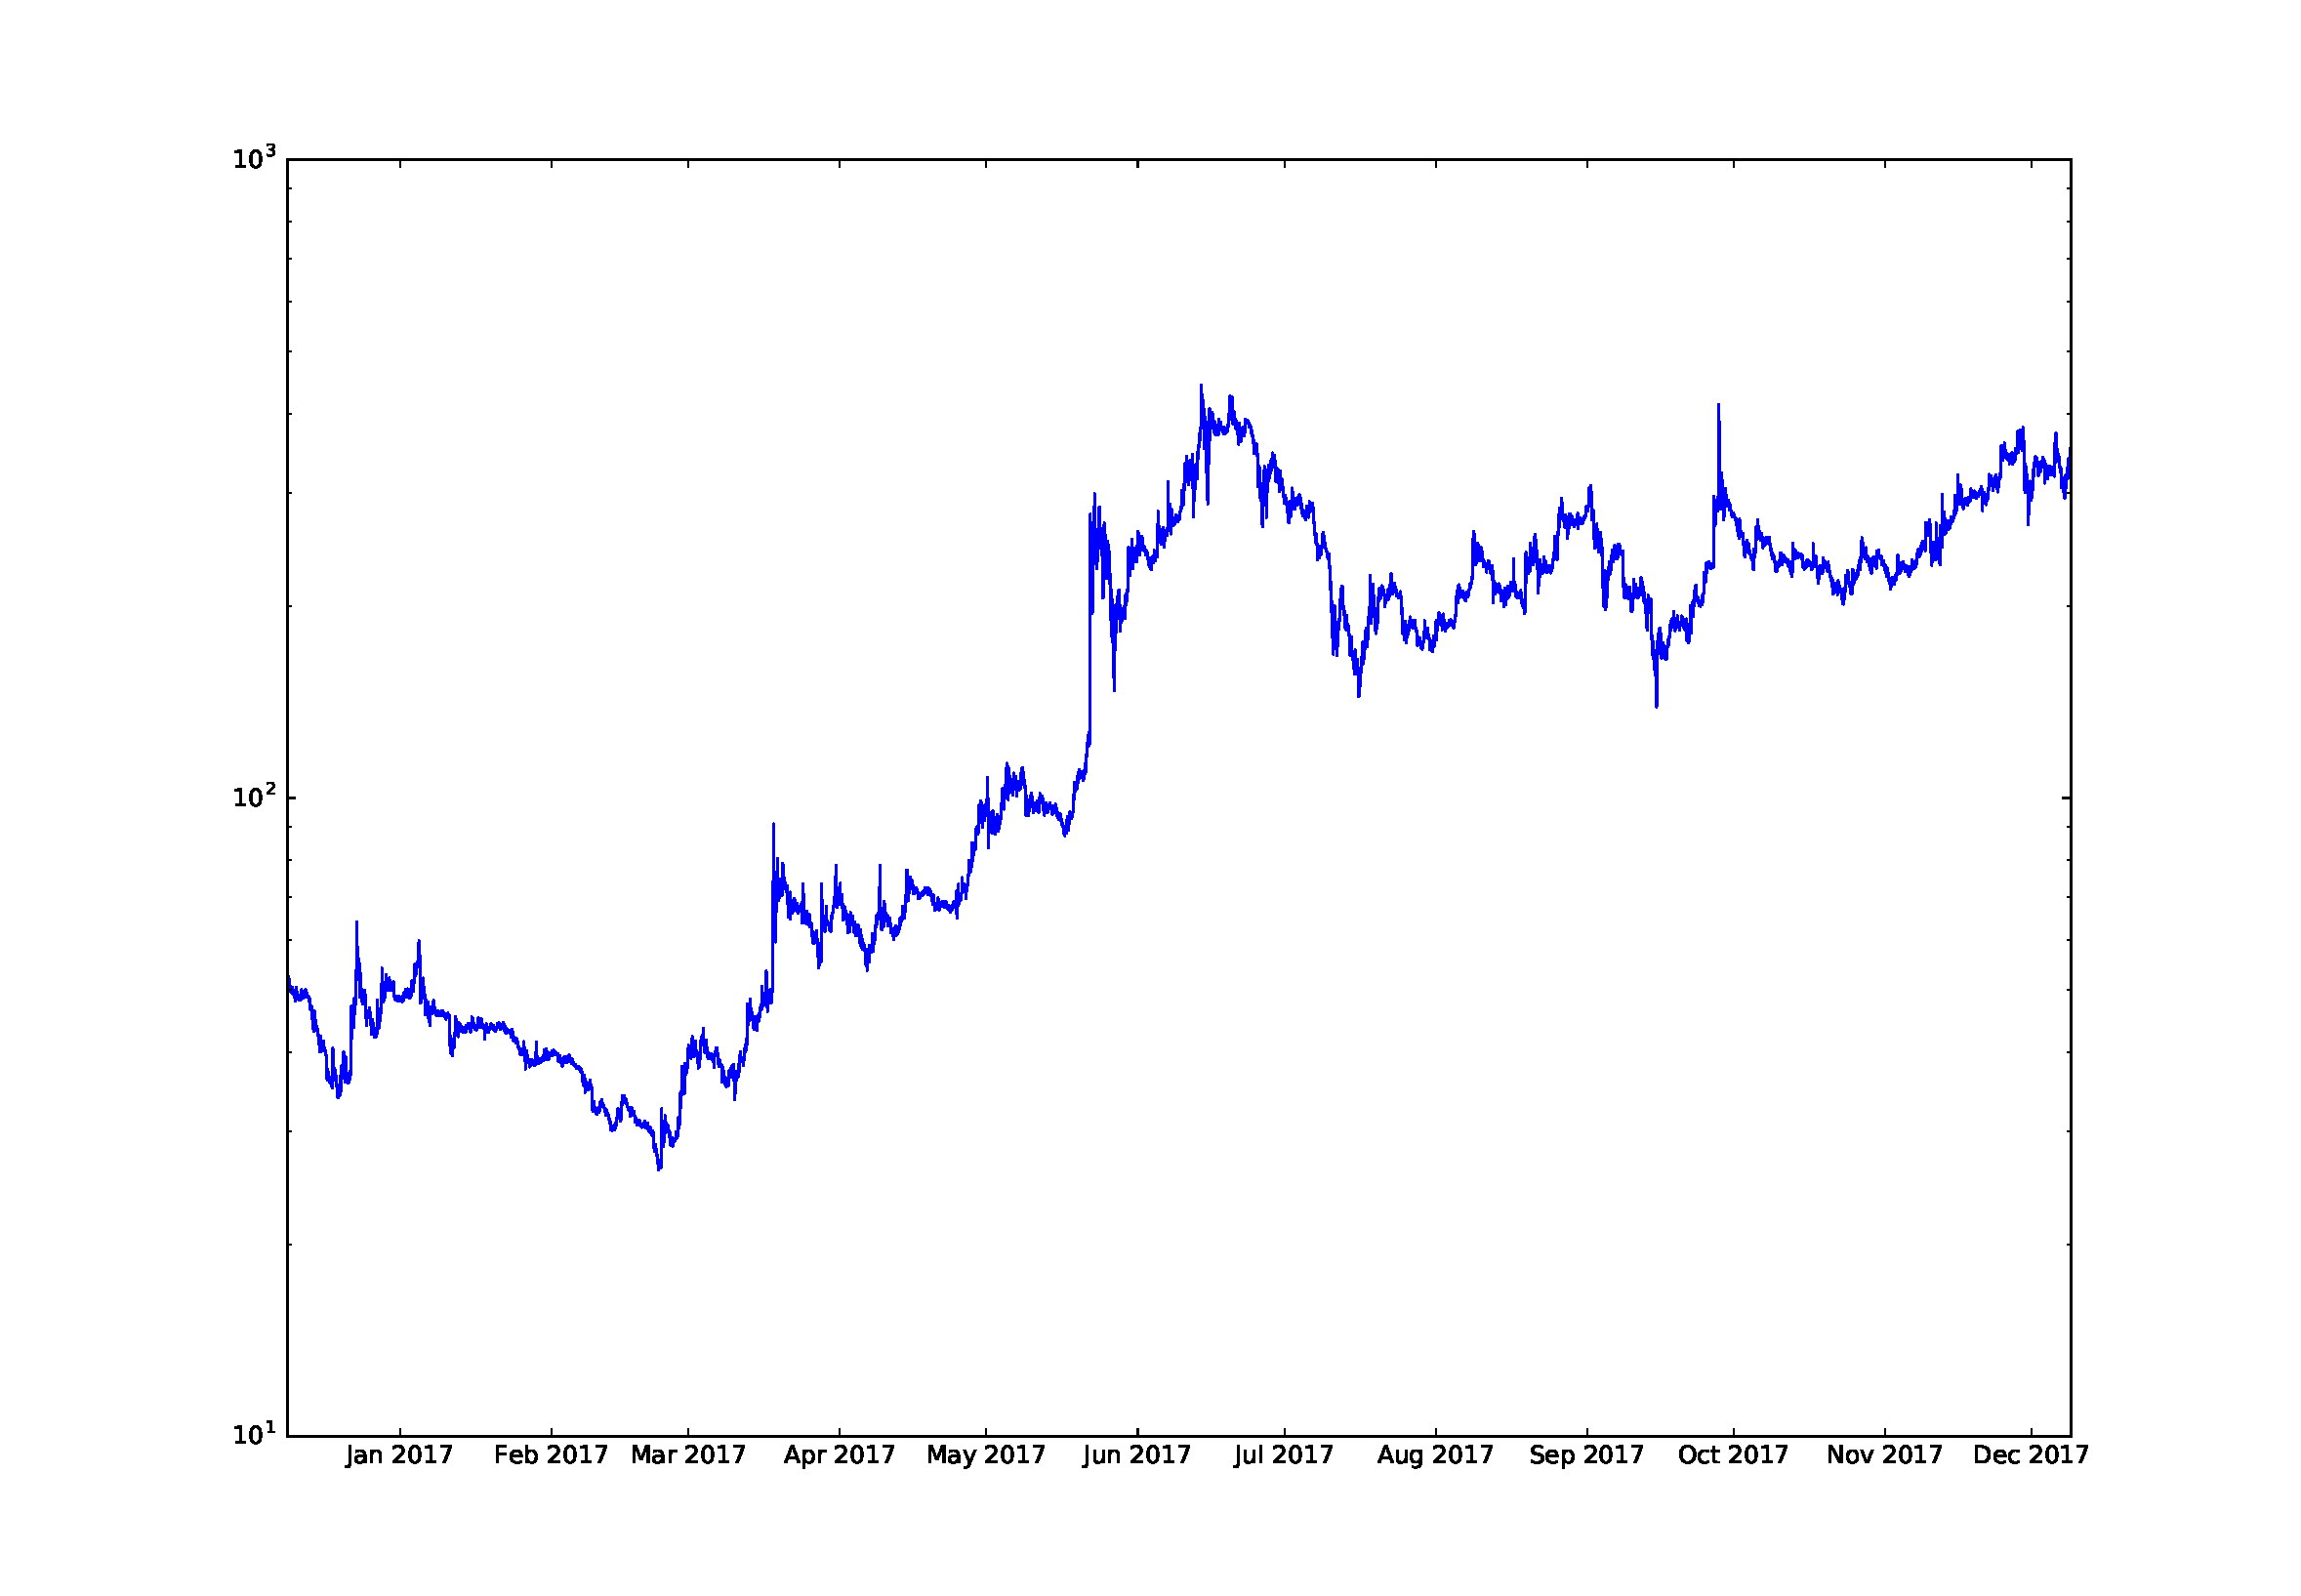
\includegraphics[width=\columnwidth]{pdf/zcash-price.pdf}
    \caption{Historical price of ZCash in logarithmic scale. Note the minimum at 23 Feb 2017}
    \label{fig:zec}
\end{figure}

ZCash is very interesting in a way that it started from an extremely high inflation (percent-wise).
This caused a short-term price drop (even though the market capitalization was growing)~(\figref{fig:zec}).
But at some point (23~Feb~2017), the price started going up.
ZCash block rewards yield $50$~ZEC every $10$~min, and ZEC supply at Feb~23 was $727$k~ZEC.
This corresponds to $360\%$~APR.
It is even more remarkable given the fact that miners who mined ZEC are probably those who dump and exchange the proceeds into something else (and also pay
electricity bills).
This gives us information about what would be the maximum allowable inflation which still doesn't create a too high down pressure for the price.

\section{Mining protocol}

Miner commits to stay available for at least certain time $T$.
If the tokens were locked for this whole time $T$ and abruptly unlocked after that, we'd have a problem with a pre-locked preallocation:
a huge increase of tokens in circulation right after the time $T$ would probably crash the market.

\begin{figure}
    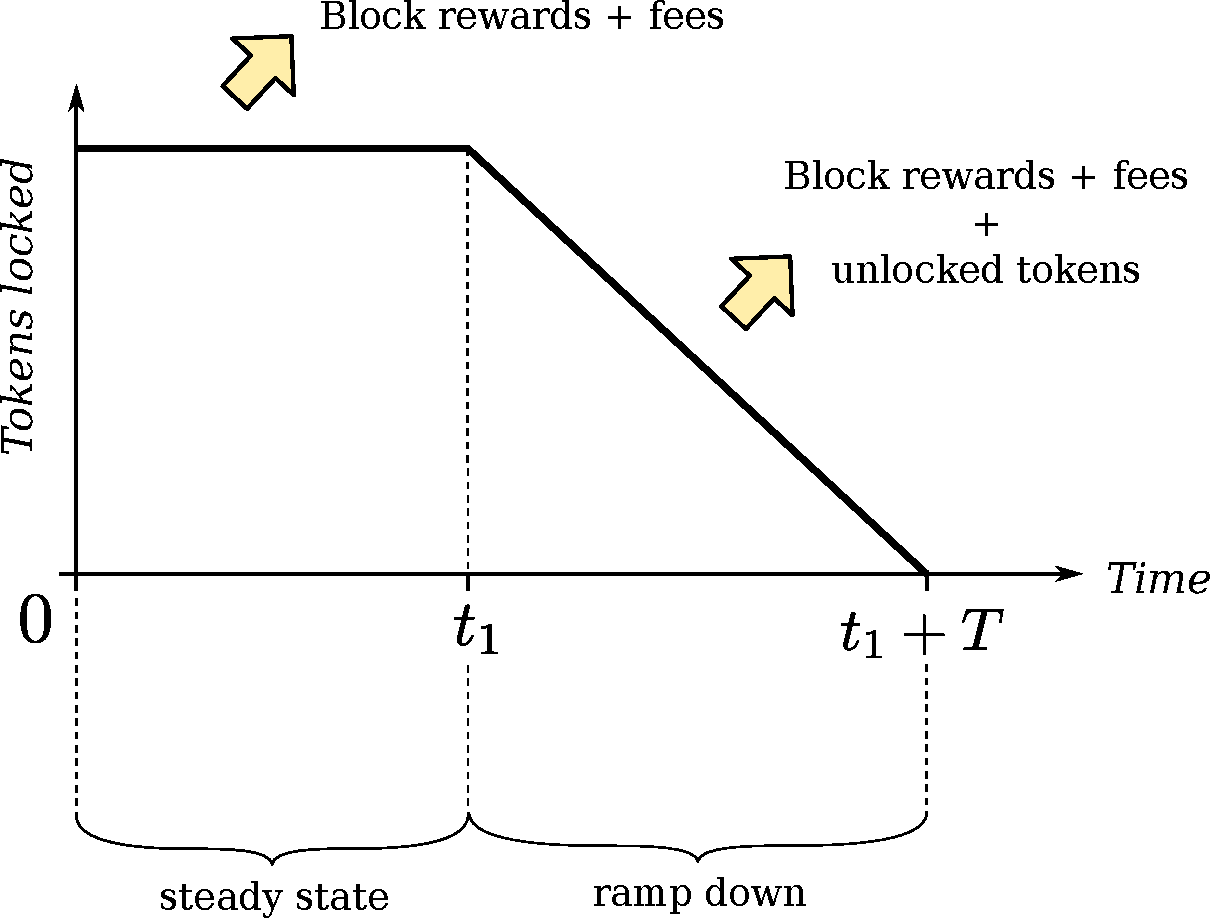
\includegraphics[width=\columnwidth]{pdf/mining-modes.pdf}
    \caption{
        Mining modes: \emph{steady state} (before $t_1$) and \emph{ramp down} (from $t_1$ till $t_1 + T$).
        The ramp down (or vesting) time $T$ is chosen by the miner (and he gets higher staking rewards when $T$ is higher).
    }
    \label{fig:mining-modes}
\end{figure}

In order to avoid that, we introduce two modes of miner operation: \emph{steady state} and \emph{ramp down}.
When miner is in steady state, his base coins stay locked.
Block rewards are created, and they aren't necessarily locked (unless the miner chooses to add newly minted coins to the locked amount).

At any point of time, the miner can switch to \emph{ramp down}.
This would start unlocking the coins which he stakes linearly, during the time $T$.
Both, \emph{steady state} mode and \emph{ramp down} starting at the point $t_1$ are shown at (\figref{fig:mining-modes}).
So, the time $T$ doesn't mean the total time during which miner's tokens are locked, but rather how quickly do the tokens get unlocked once he starts
unlocking.


\section{General inflation properties}

\subsection{Initial inflation}

Let's assume that we'll have the same number of tokens locked as DASH has: $\lambda=60\%$.
Then we'll have $1-\lambda=40\%$ in circulation.
If we have inflation rate $I$, then adjusted inflation rate (e.g. inflation as if the locked coins didn't exist) of coins in circulation will be:
\begin{equation}
    I^* = \frac{I}{1-\lambda},
\end{equation}
and we should be comparing $I^*$ with historical examples of inflation.
If we take $I^*=350\%$ (turnover point of ZCash price in an overall bullish market), the corresponding inflation $I$ will be $140\%$~APR.

To be on the safe side, we choose the starting inflation to be $I_0=100\%$~APR (or, in other words, $1/365$ per day).

\subsection{Inflation decay}

Initially, the inflation subsidises mining, but payments for re-encryption services will provide all the revenues of miners in the long run.
If all miners have the same, maximum reward rate, we choose the inflation rate to decay by factor of $2$ in $T_{1/2} = 2$ years.
The inflation, depending on time passed from the Genesis $t$, looks like:
\begin{equation}
    I(t) = I_0 \cdot 2^{-\frac{t}{T_{1/2}}} = I_0 \exp\left[ -\ln{2} \frac{t}{T_{1/2}} \right].
\end{equation}
In this case, maximum token supply (e.g. the maximum number of tokens which will ever be created) is:
\begin{equation}
    S_{\max} = S_0 + \int_0^{\infty} I(t)\, dt = S_0 + \frac{I_0 T_{1/2}}{\ln{2}} \approx 3.89\, S_0,
\end{equation}
where $S_0$ is initial number of tokens, and $I_0 = S_0$ when the former is expressed in APR.

\section{Mining strategies}

\section{Edge cases: connection problems, vesting during unlocking}

\section{TLDR}

\bibliography{mining-paper}

\end{document}
